\documentclass[a4paper,11pt]{kth-mag}
\usepackage[T1]{fontenc}
\usepackage{textcomp}
\usepackage{lmodern}
\usepackage[latin1]{inputenc}
\usepackage[swedish,english]{babel}
\usepackage{modifications}
\usepackage{hyperref}
\usepackage{graphicx}

\newcommand{\Cpp}{\texttt{C++}}
\newcommand{\Gcc}{\texttt{gcc}}
\newcommand{\Gtkmm}{\texttt{gtkmm}}
\newcommand{\Gtk}{\texttt{GTK+}}

\title{SimpleGraphPlotter v1.6}

\subtitle{Programkonstruktion f\"{o}r F, DD1342\\ Laboration 4A}
\foreigntitle{}
\author{Jim Holmstr\"{o}m\\\href{mailto:jimho@kth.se}{jimho@kth.se}}
\date{\today}
\blurb{Teacher: Ann Bengtson}

\trita{}
\begin{document}
\frontmatter
\pagestyle{empty}
\removepagenumbers
\maketitle
\selectlanguage{english}
\tableofcontents*
\mainmatter
\pagestyle{newchap}

\chapter{Introduction}
In the following part firstly the problem will be explained and secondly 
the requirements for a basic plotter will be enlisted.
A plotter is a program that can plot functions from strings which defines the 
functions by ordinary math syntax. 
This project uses \Cpp~ programming language and the 
\Gtkmm\footnote{Documentation, binaries and source can be found at: 
\href{http://www.gtkmm.org}{www.gtkmm.org}} wrapper for the 
\Gtk\footnote{Documentation, binaries and source can be found at: 
\href{http://www.gtk.org}{www.gtk.org}} toolkit to generate the graphical user interface. 
It is compiled with the \texttt{GNU} \Gcc compiler.

\section{Requirements}
A few basic things is needed to have a functioning math plotter:
\begin{enumerate}
\item Define a function given ordinary math syntax.
\item Parse the inputed function and plot it accordingly.
\item Add/Remove functions from plotarea.
\item Plotarea should be scrollable both vertical and horizontal.
\item Range should be fixed to the unit-cube.
        \footnote{This restriction will be handled in section \ref{sec:scope}}
\item Display axis of the plot.
\item Parser must be properly tested.
\end{enumerate}

\section{Scope}
\label{sec:scope}
The amount of functionality that is possible to put in a system like this is
almost endless so a few delimitations has to be made in order to complete the project.
The currently biggest restriction to the plotter is the lack of 
ability to zoom or change the range from the unit-cube.
No support for parametric nor complex functions.
\footnote{
    Since no native support in \Cpp~ for complex numbers which means 
    all the basic math functions would have to be rewritten in order for this to work.
}

\section{Assistance}
Besides the reference manuals for \Gtkmm ~ no external help for this project was
received.

\chapter{Structure}
An basic overview of the structure can be seen in figure \ref{fig:UML}, all
parts will then be enlisted and explained in a \verb+javadoc+ like manner.
\begin{figure}[ht]
\begin{center}
    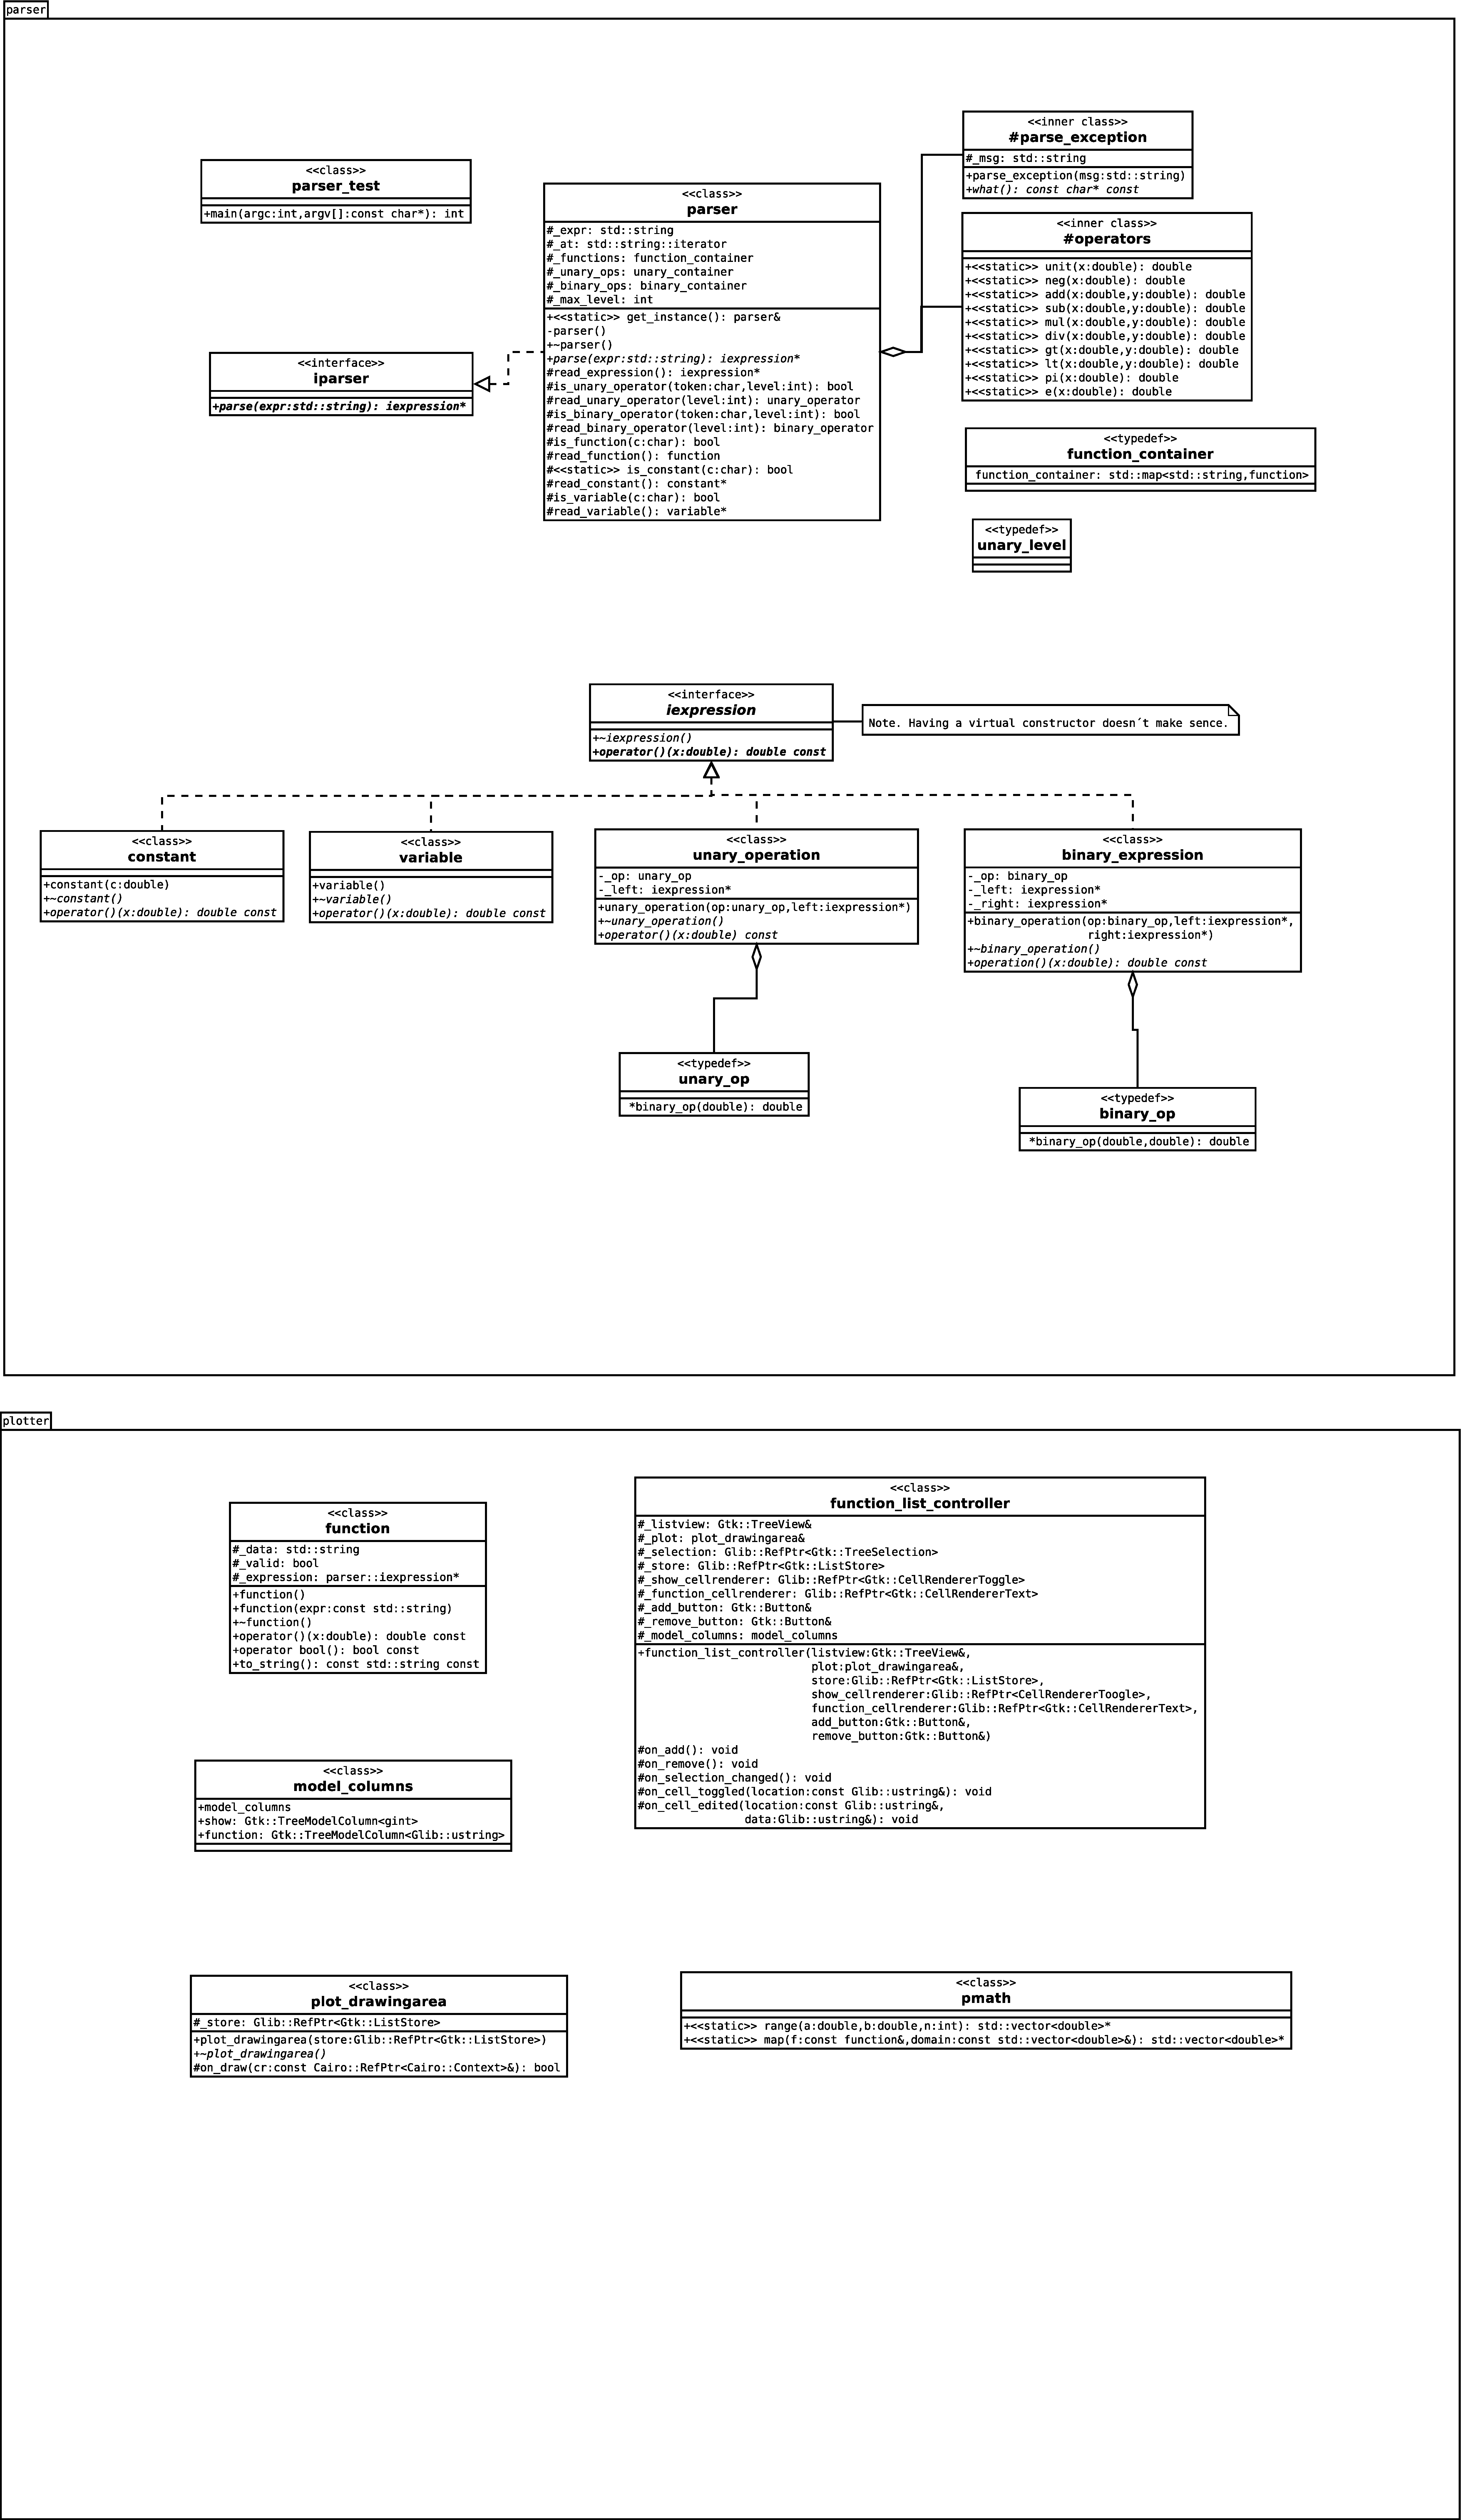
\includegraphics[width=\textwidth]{uml.pdf}
    \caption{\small{An UML showing the structure and the enclosure.}}\label{fig:UML}
\end{center}
\end{figure}

\section{Parser}
The parser code can be divided into to parts the algorithm code, that is the 
actual parser, and the data structure in the form of a parse tree.

\begin{figure}[ht]
\begin{center}
    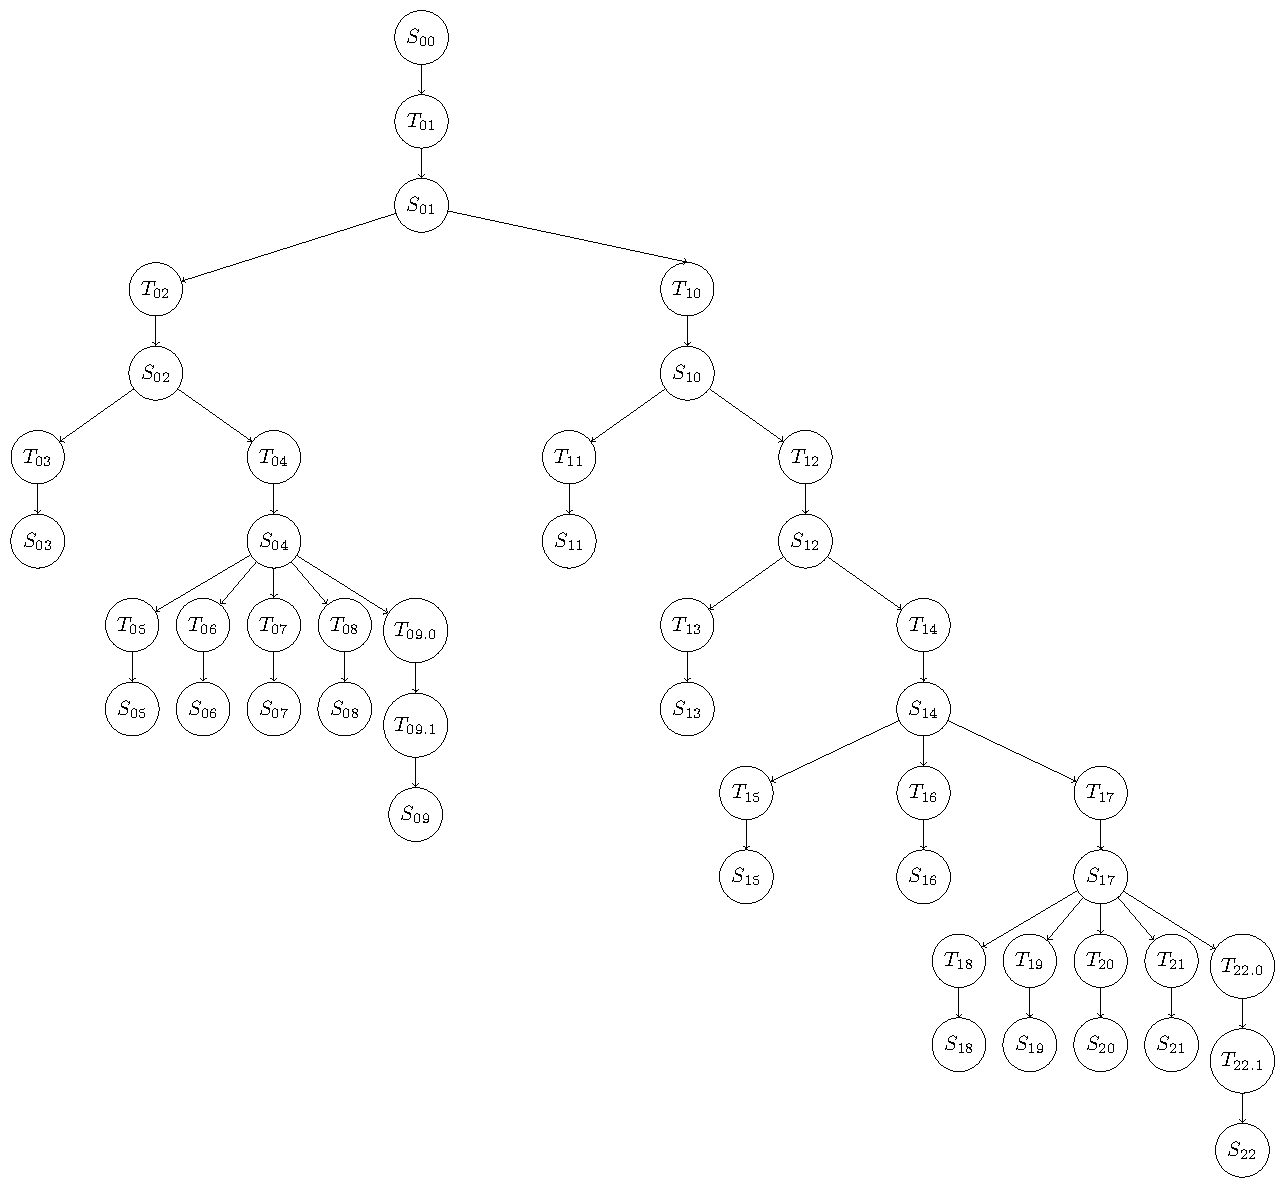
\includegraphics[width=\textwidth]{parse-tree.pdf}
    \caption{\small{
        An example of the parse tree for the
        expression \texttt{sin(x+2)*(x-1)}\texttt{\^~}\!\!\texttt{5}.
    }}
   \label{fig:parsetree}
\end{center}
\end{figure}

%TODO order all sections/subsections in descending order of importance (tex. parse should be placed first)
\subsection{parser}
%<basic description of the class>
%<example of a parse tree, with all the different components like pharanthesis
%and functions, binary and unary operators. and how they are really handled in
%the parsing>

\begin{description}
    \item[public parse(expr : std::string)] 
        Test explain test test test
        \begin{description}
            \item[Parameters:]~\\
                \verb+expr+ - test test
            \item[Returns:]~\\
                \verb+iexpression*+ - test test

        \end{description}
        Public <basic description of the function> TODO should i perhaps move the arguments/return as i doxygen to their own posts?
\end{description}
\subsubsection{parse\_exception}
\subsubsection{operators}

%\subsection{function\_container}
\subsection{unary\_level}
what is this used for?
\subsection{iexpression...}

\section{Plotter}
...
<images with the different parts highlighted with a red border, that is the parts being described at the moment>
especially point out the inheritance in the custom widgets.

\chapter{Results and Discussion}

\section{Results}
<<screenshots>>
Runned trough valgrind, results?.

\section{Discussion}
Problems with the unofficial \Cpp wrapper \Gtkmm, only used it to avoid missing out inheritance, polymorphism and to get it compatible with the standard \Cpp Library. 
 


\end{document}
